\chapter{Results and Statistical Analysis}\label{ch:results}

Every number in this chapter was recomputed from the raw per-trial records during the
preparation of this report, not copied from an earlier document. The recomputation script is
\code{experiments/validate\_figures.py}, which reads \code{ablation.jsonl} rather than the
derived summary.

\section{Statistical treatment}

Three decisions govern every test reported below.

\textbf{Interval estimates.} Proportions are reported with 95\% Wilson score intervals rather
than the normal approximation, because several arms sit at or near $p=0$ or $p=1$ where the
normal interval is degenerate and can extend outside $[0,1]$. Intervals are clamped at the unit
bounds.

\textbf{Hypothesis tests: the design is matched pairs.} Every arm runs on the same 300 seeds with
the same seed-to-attack-rate mapping, so each seed yields a matched pair and only discordant pairs
carry information. The primary test is the exact one-sided McNemar test. An earlier version of
this report used Fisher's exact test, which assumes two independent samples --- an assumption this
design does not satisfy, and which overstated the evidence by roughly fifty orders of magnitude in
one comparison. Fisher figures are retained only as a labelled sensitivity analysis. $\chi^2$ is
avoided because several tables contain zero cells.

\textbf{Clustered observations.} The availability metric takes five operator attempts per trial,
and those five share that trial's token-bucket phase: 231 of 250 rate-limiter trials admitted
either all five or none. The intra-cluster correlation is 0.669, a design effect of 3.68, so 1,250
attempts carry the information of about 340 independent ones. The attempt-level proportion is
reported because it is what an operator experiences; the test is at the trial level, which is the
independent unit.

\textbf{Where no test is reported.} No hypothesis test is applied to a quantity whose variance
is identically zero by construction. The simulation harness advances a logical clock, so the
safety latency is the same constant — 151\,ms, being the sensor confirmation window plus the
loop period — in every trial. A test on two constant-valued samples is trivially satisfied and
carries no information. The pre-registered test for the hardware measurement is in
Appendix~\ref{app:hardware} and was committed before any data existed.

Because every arm is a fixed, pre-declared configuration rather than a selected subset, no
multiplicity correction is applied. This is noted so a reader can judge it rather than infer it.

\section{Trial accounting}

\begin{longtable}{@{}p{0.07\textwidth}p{0.34\textwidth}p{0.20\textwidth}p{0.29\textwidth}@{}}
\toprule
\textbf{ID} & \textbf{Experiment} & \textbf{Scale} & \textbf{Artefact} \\
\midrule
\endhead
E1 & Campaign, baseline build        & 3{,}000 trials        & \code{summary.json} \\
E2 & Campaign, hardened build        & 3{,}000 trials        & \code{summary.json} \\
E3 & Command-path ablation           & 3{,}600 trials        & \code{ablation.jsonl} \\
E4 & Host-build fuzzing              & 3{,}000{,}000 iter.   & \code{fuzz.json} \\
E5 & Detector sensitivity            & 180 grid cells        & \code{sensitivity.jsonl} \\
E6 & Live-broker access control      & 8 scenarios           & \code{broker\_acl.jsonl} \\
E7 & Open-source corpus              & 135 projects          & \code{corpus.json} \\
E8 & Trace conformance               & 19{,}529 transitions  & \code{test\_conformance.py} \\
E9 & Model checking                  & 25 and 660 states     & \code{formal/} \\
\midrule
\multicolumn{2}{@{}l}{\textbf{Total adversarial trials}} & \textbf{9{,}600} &
3{,}000 + 3{,}000 + 3{,}600 \\
\bottomrule
\end{longtable}

\section{E1 and E2: the adversarial campaign}

Across 6,000 trials \textbf{no adversary disarmed the device and no safety invariant was
violated.}

Without command authentication the adversary changed the system state in all 2,500 flooded
trials; with authentication, in none. The availability result is the more informative of the
two: with authentication a legitimate command took effect in all 3,000 trials regardless of
attack rate, while in the baseline, flooding starved it in every flooded trial.

\textbf{What this does not show.} It shows nothing about timing. The safety latency is a
constant in this environment, so the campaign establishes that the \emph{logic} holds under
adversarial load and nothing about whether the \emph{silicon} does.

\section{E3: the command-path ablation}\label{sec:res-ablation}

\subsection{The six command-path designs}

Figure~\ref{fig:ablation} shows three properties across the six designs.

\begin{figure}[htbp]
\centering
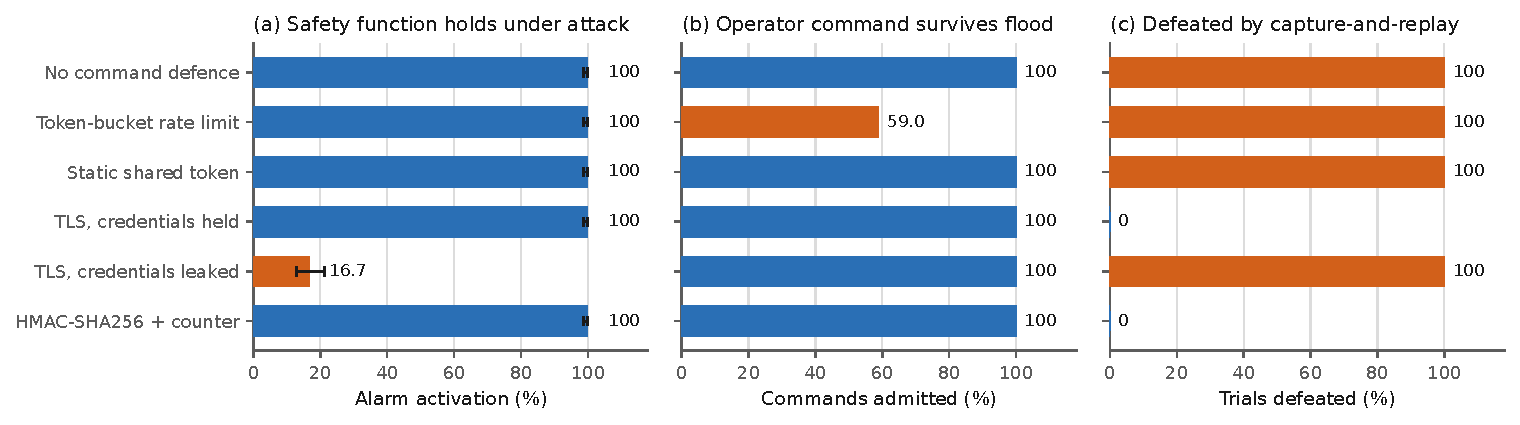
\includegraphics[width=\textwidth]{ablation_results.pdf}
\caption[Command-path ablation results]{Command-path ablation. 300 trials per bar in panels (a)
and (c); 1,250 operator attempts per bar in panel (b). Whiskers in (a) are 95\% Wilson score
intervals. Panel (c) inverts the reading: there a high value is the failure, so the colour rule
inverts with it, and blue continues to mean ``this design holds the property''.}
\label{fig:ablation}
\end{figure}

\begin{longtable}{@{}p{0.27\textwidth}rrrr@{}}
\toprule
\textbf{Design} & \textbf{Alarm} & \textbf{95\% Wilson} & \textbf{Avail.} & \textbf{Replay} \\
\midrule
\endhead
No command defence        & 300/300 & [98.7, 100.0] & 100.0\% & 100\% \\
Token-bucket rate limit   & 300/300 & [98.7, 100.0] & \textbf{59.0\%} & 100\% \\
Static shared token       & 300/300 & [98.7, 100.0] & 100.0\% & 100\% \\
TLS, credentials held     & 300/300 & [98.7, 100.0] & 100.0\% & 0\% \\
TLS, credentials leaked   & \textbf{50/300} & \textbf{[12.9, 21.3]} & 100.0\% & 100\% \\
HMAC-SHA256 + counter     & 300/300 & [98.7, 100.0] & 100.0\% & 0\% \\
\bottomrule
\end{longtable}

\subsection{Three findings}

\textbf{The three properties fail independently.} This is the central result of the ablation and
it is not what one would assume. The rate limiter preserves the safety function and replay
resistance is unchanged at 100\% defeated, yet it costs \textbf{41\% of legitimate operator
commands}. The static token does the reverse: every operator command is admitted and replay
resistance is nil. Only the counter-bound message authentication code holds all three. A designer who treats
``security'' as one property will choose badly here.

Paired by seed at the trial level, 112 pairs are discordant and all favour the authenticated
design: McNemar exact, one-sided, $p = 1.9 \times 10^{-34}$. (Fisher, ignoring both the pairing
and the clustering, would give $3.5 \times 10^{-184}$.)

The aggregate is also the wrong summary of the limiter's own behaviour, and the per-rate figures
are what a reader needs: 82 of 250 operator attempts admitted at 10\,commands/s, \textbf{0 of 250
at 100\,commands/s}, 155 of 250 at 1,000, and all 250 at both 5,000 and 20,000. The cost is not
monotonic in attack intensity and the extremes are the benign cases, because an arrival finding
the bucket below the admission threshold is rejected \emph{without consuming a token}: an extreme
flood pins the bucket just under the threshold and leaves enough refill for the next legitimate
arrival. A defender who tunes the limiter against the worst flood they can generate measures no
availability cost at all, and meets the complete lockout in the field two orders of magnitude
lower.

\textbf{Transport security alone is contingent on credential secrecy.} With credentials held,
TLS gives 100\% alarm activation and no replay. With a single credential leaked, alarm
activation falls to 16.7\%, 95\% Wilson [12.9, 21.3], and the adversary disarms the device in
246 of 300 trials. Of the 300 matched pairs, 250 are discordant and every one lost the alarm when
the credential leaked, with none gaining it: McNemar exact, one-sided,
$p = 5.5 \times 10^{-76}$. (Fisher would give $9.8 \times 10^{-119}$.)

\textbf{The alarm still firing is not the same as the system being secure.} In the
\code{none}, \code{ratelimit} and \code{token} arms the alarm fires in all 300 trials, and all
three are completely defeated by capture-and-replay. Panel (a) read alone would suggest that no
command defence is as safe as a message authentication code. Panel (c) is what prevents that
reading, and this is why the figure has three panels rather than one.

\section{Broker authorisation against message authentication}\label{sec:res-credential}

\subsection{The nine-cell matrix}

Figure~\ref{fig:credential} indexes outcomes by \emph{which secret the adversary holds} rather
than by mechanism, because that is the comparison the design question requires.

\begin{figure}[htbp]
\centering
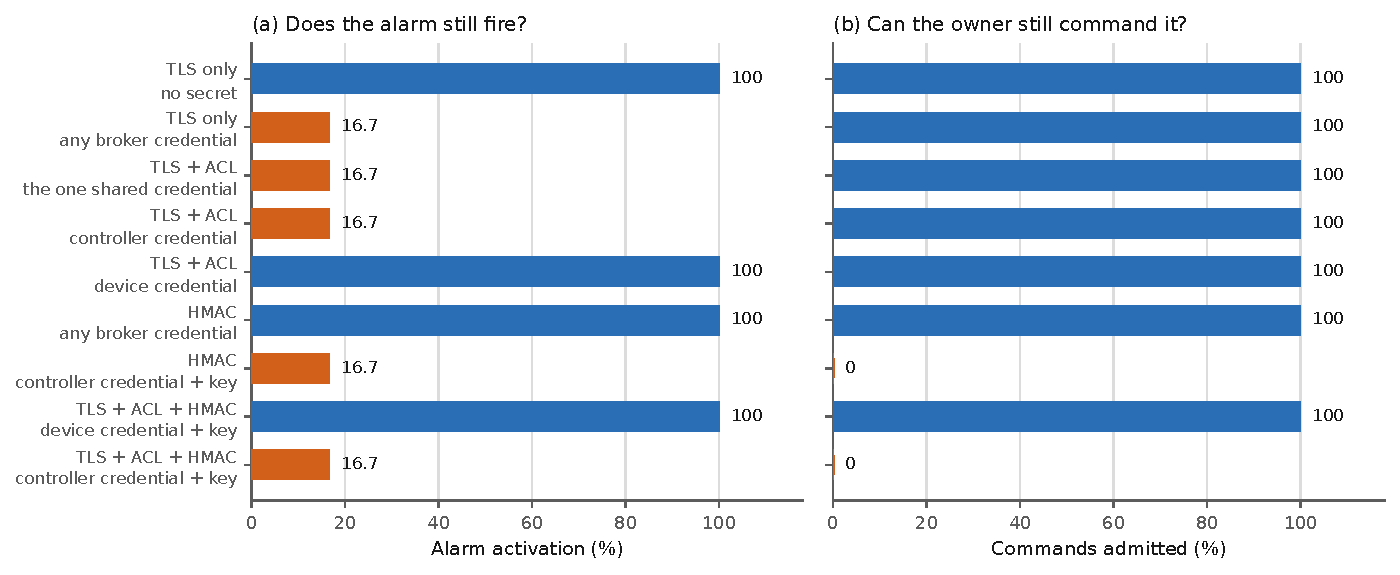
\includegraphics[width=\textwidth]{credential_matrix.pdf}
\caption[Security compromise comparison]{Alarm activation and operator availability for nine
combinations of control and compromised secret. The bottom row is the layered build under a
compromised controller host: it fails, and is drawn at the same weight as every other row.}
\label{fig:credential}
\end{figure}

\begin{longtable}{@{}p{0.19\textwidth}p{0.26\textwidth}rrr@{}}
\toprule
\textbf{Control} & \textbf{Compromise} & \textbf{Alarm} & \textbf{Operator admitted} &
\textbf{Disarms} \\
\midrule
\endhead
TLS only        & none                       & 300/300 & 1250/1250 & 0 \\
TLS only        & any broker credential      & 50/300  & 1250/1250 & 246 \\
TLS + ACL       & the one shared credential  & 50/300  & 1250/1250 & 246 \\
TLS + ACL       & controller credential      & 50/300  & 1250/1250 & 246 \\
TLS + ACL       & device credential          & 300/300 & 1250/1250 & 0 \\
HMAC + counter  & any broker credential      & 300/300 & 1250/1250 & 0 \\
HMAC + counter  & controller cred.\ + key    & 50/300  & \textbf{0/1250} & 234 \\
TLS+ACL+HMAC    & device cred.\ + key        & 300/300 & 1250/1250 & 0 \\
TLS+ACL+HMAC    & controller cred.\ + key    & 50/300  & \textbf{0/1250} & 234 \\
\bottomrule
\end{longtable}

\subsection{Neither control dominates}

The matrix shows that broker authorisation and application-layer authentication fail under
\emph{different} compromises, and that neither contains the other.

The access control list contains a compromised \emph{device} credential, which the message
authentication code does not — because the command key lives in the same flash image as the
device's broker credential, so a flash dump yields both. Conversely the message authentication
code contains a compromised \emph{controller} credential, which the access control list cannot
— because the list must permit that identity to publish commands.

\subsection{An unanticipated negative result: owner lockout}

Two rows show \textbf{0 of 1,250} operator commands admitted. This was not predicted.

Under key compromise the adversary signs commands with a counter far above the operator's. The
device persists that counter, as it must in order to resist replay. Every subsequent legitimate
command then carries a lower counter and is correctly rejected as a replay. The mechanism that
defeats capture-and-replay has become a lockout against the legitimate owner.

\textbf{The mechanism is not new; the measurement is.} A literature check carried out for this
report found the mechanism stated as background in work on ZigBee replay attacks: Wara and
Yu~\cite{wara2020} note that an attacker can set a device's frame counter above its normal value
so that subsequent lower-counter frames are discarded. They state it in passing, without a
citation and without an experiment, and their own measurements go the other way --- they test
whether raising a captured frame's counter lets a \emph{replay} succeed, not whether it blocks
legitimate traffic.

What this work adds is therefore not the observation but the quantification and the attribution:
the lockout is complete rather than partial (0 of 1,250), it arises from a design decision made
for a defensible reason, and it shows that replay resistance and owner availability are coupled
under key compromise rather than independent. An earlier draft of this report claimed the
mechanism had not been reported at all. That claim was wrong and has been withdrawn.

\subsection{An overclaim found by measuring the missing arm}\label{sec:res-overclaim}

An earlier draft of this work stated that the layered configuration ``survives every case''.
That statement was false, and it was found to be false by running the arm the draft had not run.

The layered configuration survives every single-secret compromise \emph{and} a device flash
dump. It falls to a compromised controller host. Since the flash dump requires physical access
and the controller-host compromise does not, the configuration survives the expensive scenario
and fails the cheap one. Figure~\ref{fig:security} draws both.

\begin{figure}[htbp]
\centering
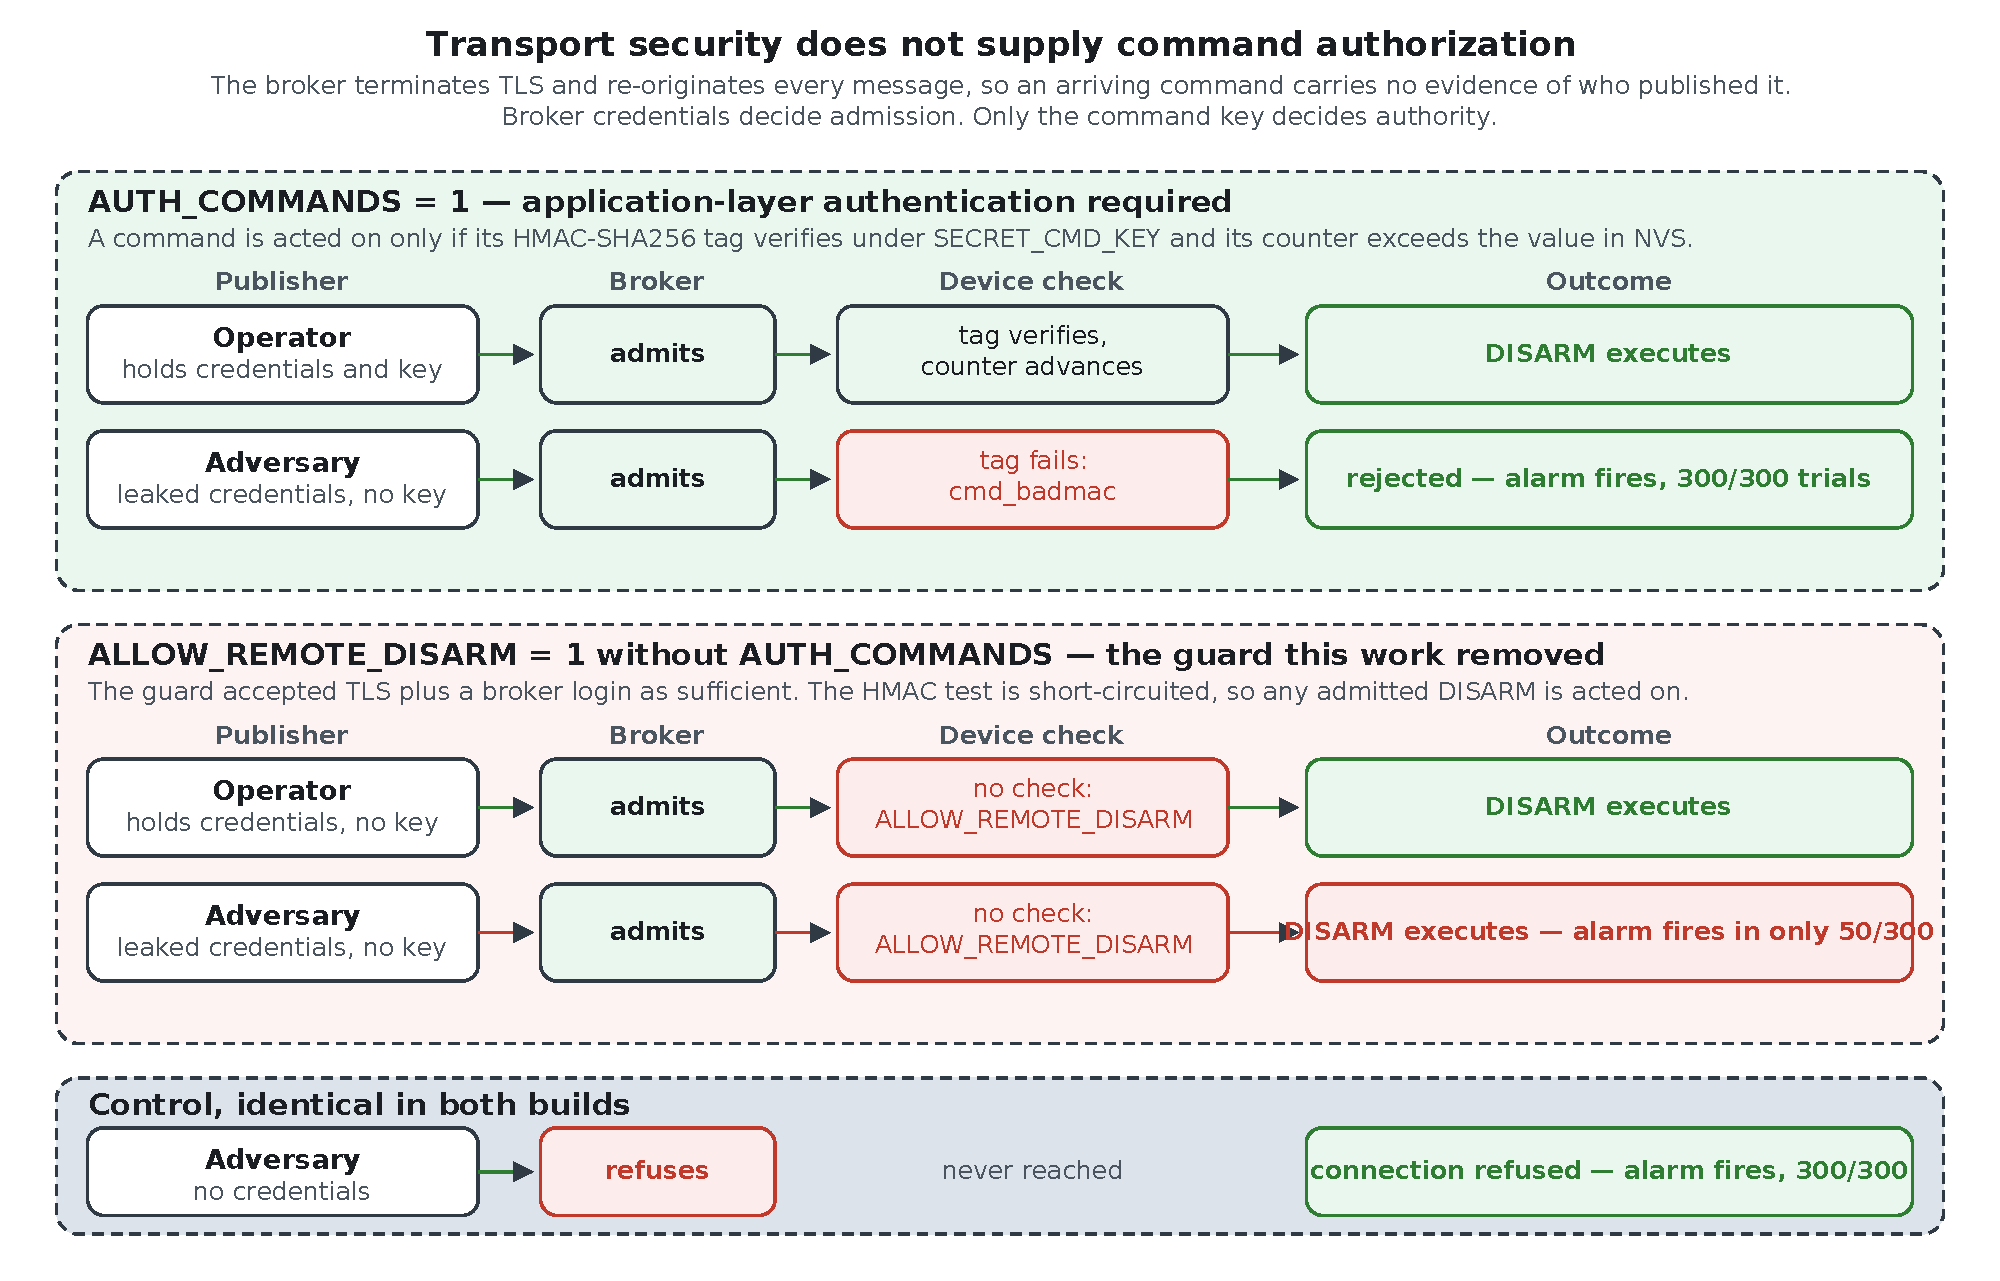
\includegraphics[width=\textwidth,height=0.74\textheight,keepaspectratio]{security_paths.pdf}
\caption[Transport security versus command authorisation]{Where broker credentials decide
admission and where the command key decides authority. The third row of the upper panel is the
compromised controller host, holding both a permitted credential and the key: neither layer
refuses it, and the alarm fires in only 50 of 300 trials.}
\label{fig:security}
\end{figure}

\section{E6: results against a live broker}\label{sec:res-broker}

All eight scenarios were run against Mosquitto 2.0.18 over TLS 1.2 with a private certificate
authority. The verdicts reproduce: re-running the experiment on a freshly installed broker in a
clean environment during the preparation of this report returned verdicts identical to the
committed run, with only the broker's own log timestamps and random client identifiers
differing.

\begin{longtable}{@{}llccc@{}}
\toprule
& \textbf{Adversary identity} & \textbf{Connected} & \textbf{Delivered} &
\textbf{Would execute} \\
\midrule
\endhead
\multicolumn{5}{@{}l}{\textit{Per-client access control list}} \\
control & controller (legitimate)      & yes & yes & yes \\
A       & no credentials               & \textbf{no} & no  & no \\
C       & controller credential        & yes & yes & \textbf{yes} \\
D       & device credential            & yes & \textbf{no}  & no \\
E       & device credential + key      & yes & \textbf{no}  & no \\
E$'$    & controller credential + key  & yes & yes & \textbf{yes} \\
\midrule
\multicolumn{5}{@{}l}{\textit{Single shared credential}} \\
control & controller, shared ACL       & yes & yes & yes \\
B       & shared credential            & yes & yes & \textbf{yes} \\
\bottomrule
\end{longtable}

\textbf{E and E$'$ are the decisive pair.} The \emph{same valid signature}, carried by the
device identity, is not delivered; carried by the controller identity, it is. What stops
scenario E is therefore the access control list and not the signature. This is the result that
could not be established by modelling alone, and it is the reason the experiment was worth
running against real broker software.

\section{E5: detector parameter sensitivity}

The sweep produced a correction rather than a confirmation. At the detector's original shipped
configuration — threshold 8 frames within a 2,000\,ms window — the detector fired in
\textbf{1,597 of 2,000} benign ten-minute runs (79.85\%). That is not a detector; it is an
alarm that reports almost continuously under normal conditions.

The firmware now ships \code{DEAUTH\_THRESHOLD = 12}. The sweep is reported because the
original value was wrong by a wide margin and the sweep is what revealed it.

\section{E4: fuzzing}

3,000,000 iterations across six input classes under both sanitizers produced \textbf{no crash,
no sanitizer report and no accepted input}: no input changed state or advanced the counter
without a valid tag.

\textbf{What this is evidence of, and what it is not.} It is evidence of memory safety and
parser robustness. It is \emph{not} independent evidence of authentication soundness: against a
128-bit tag, zero forgeries in three million attempts is the expected outcome whether the
implementation is sound or not, since the probability of a chance forgery is $2^{-128}$.

\section{E7: the corpus study, and a negative result}\label{sec:res-corpus}

\subsection{Rule 1 found nothing}

The precise guard rule returned \textbf{zero hits across 135 projects}.

That is reported as a zero. \textbf{No claim is made that the pattern is widespread}, and the
finding remains a single-system case study.

The zero is also explained rather than left bare. Only 30 of the 135 projects both subscribe to
MQTT and contain any application-authentication identifier at all, and reading those shows that
most matches sit in vendored third-party code rather than in the project's own command path.
The corpus is biased by construction — 22 fixed queries, a minimum of 3 stars, a size cap of
80\,MB, archived repositories and forks excluded — and those criteria are recorded with the
rejection counts in \code{corpus.json}.

\subsection{The rule was wrong at first}

This matters for the credibility of the zero. The rule initially returned zero against
\emph{this project's own pre-repair guard}, because it treated any mention of the
authentication identifier as evidence that authentication was required — and in the defective
guard that identifier appears \emph{negated}. Until this was found, the zero result was
meaningless.

Eight controls now exist as a direct consequence, including the project's own pre-repair guard
as a positive control and its repaired guard as a negative control. All eight pass.

\subsection{Rule 2 and the nine confirmed projects}

The looser heuristic flagged 18 of 135. Reading all 18 by hand gave 9 confirmed and 9 false
positives.

This is reported as an \textbf{existence claim and not a rate}. The rule over-counts monitoring
projects by roughly half and under-counts non-GPIO actuation by an unknown amount: three of the
nine confirmed cases actuate through Modbus, RF or serial frames and were caught only by an
incidental GPIO write. The 18/135 figure is therefore not a prevalence estimate and must not be
read as one.

\section{E8 and E9: conformance and model checking}

\textbf{Trace conformance.} 19,529 firmware transitions across three ablation modes — 7,044,
5,282 and 7,206 — checked against the transition relation parsed from \code{AlarmFSM.tla}.
\textbf{Zero disallowed transitions.} The negative control confirms that a forbidden
\code{Disarmed} $\rightarrow$ \code{Alarm} transition \emph{is} rejected, which is what makes
the 19,529 meaningful: a checker that accepts everything would also report zero violations.

\textbf{Model checking.} \code{AlarmFSM}: 166 states generated, 25 distinct.
\code{Isolation}: 2,686 generated, 660 distinct. Both exhaustive. The third configuration and
its purpose are the subject of Chapter~\ref{ch:formal}.

\section{Summary of statistical values}

Every value below was recomputed from the raw records during the preparation of this report.

\begin{longtable}{@{}p{0.47\textwidth}p{0.22\textwidth}p{0.21\textwidth}@{}}
\toprule
\textbf{Claim} & \textbf{Recomputed} & \textbf{Status} \\
\midrule
\endhead
Leaked-credential alarm activation 16.7\%        & 50/300 = 16.67\%        & exact \\
95\% Wilson interval [12.9\%, 21.3\%]            & [12.9, 21.3]            & exact \\
Rate limiter admits 59.0\% of operator commands  & 737/1250 = 59.0\%       & exact \\
McNemar exact (paired), availability             & $1.93\times10^{-34}$    & exact, primary \\
McNemar exact (paired), transport arms           & $5.53\times10^{-76}$    & exact, primary \\
Intra-cluster correlation, 5 attempts per trial  & 0.669 (design eff.\ 3.68) & exact \\
Fisher exact, unpaired sensitivity only          & $3.53\times10^{-184}$, $9.83\times10^{-119}$ & superseded \\
Adversary disarms in 246 of 300 trials           & 246                     & exact \\
Owner lockout 0 of 1,250                         & 0/1250                  & exact \\
Detector default fired in 1597/2000 benign runs   & 1597/2000 = 79.85\%     & exact \\
TLC distinct states, 25 and 660                  & 25 and 660              & exact \\
Trace transitions, 19,529                        & 7044+5282+7206          & exact \\
\bottomrule
\end{longtable}
